\title{Madrid Rent Prices}
\maketitle

\section{Contexto}

El contexto de esta práctica se basa en el estudio y el análisis del estado de la situación actual del alquiler,
 ya que, como se ha vivido en los últimos años existe una gran demanda ligado a su correspondiente aumento de 
 precios. Para esto se ha trabajado con la web \href{https://www.fotocasa.es/es/}{Fotocasa} a través de la 
 herramienta Selenium y centrándonos exclusivamente en la ciudad de Madrid.

A pesar de centrarnos solamente en la web \href{https://www.fotocasa.es/es/}{Fotocasa} todo el código desarrollado 
se ha enfocado para extrapolar la metodología aplicada a otras web con similar contexto.

\section{Título}

A partir del contexto anterior se ha establecido el nombre \textit{\textbf{Madrid Rent Prices}} 
para el conjunto de datos generado.

\section{Descripción del dataset}

Como se puede intuir, cada elemento del conjunto representa una casa/piso de alquiler 
en \href{https://www.fotocasa.es/es/) y sus correspondientes atributos los cuales se describirán 
en las siguientes secciones. Estos elementos se han obtenido en diversos días durante el mes de 
abril de este año (2022}{Fotocasa} para tener una variabilidad de los cambios ocurridos en determinados 
periodos de tiempo.

\section{Representación gráfica}

A continuación se ve una representación del proyecto completo. Se obtienen los datos de 
\href{https://www.fotocasa.es/es/}{Fotocasa} mediante Selenium y el código realizado en Python. 
Por un lado, guarda los datos en la base de datos, con la opción de ejecutar el posterior código 
para transformar estos datos en formato \textit{CSV} y por otro lado se puede conectar con Google Drive 
para guardar las imágenes en una carpeta determinada:

\begin{figure}[H]
      \centering
      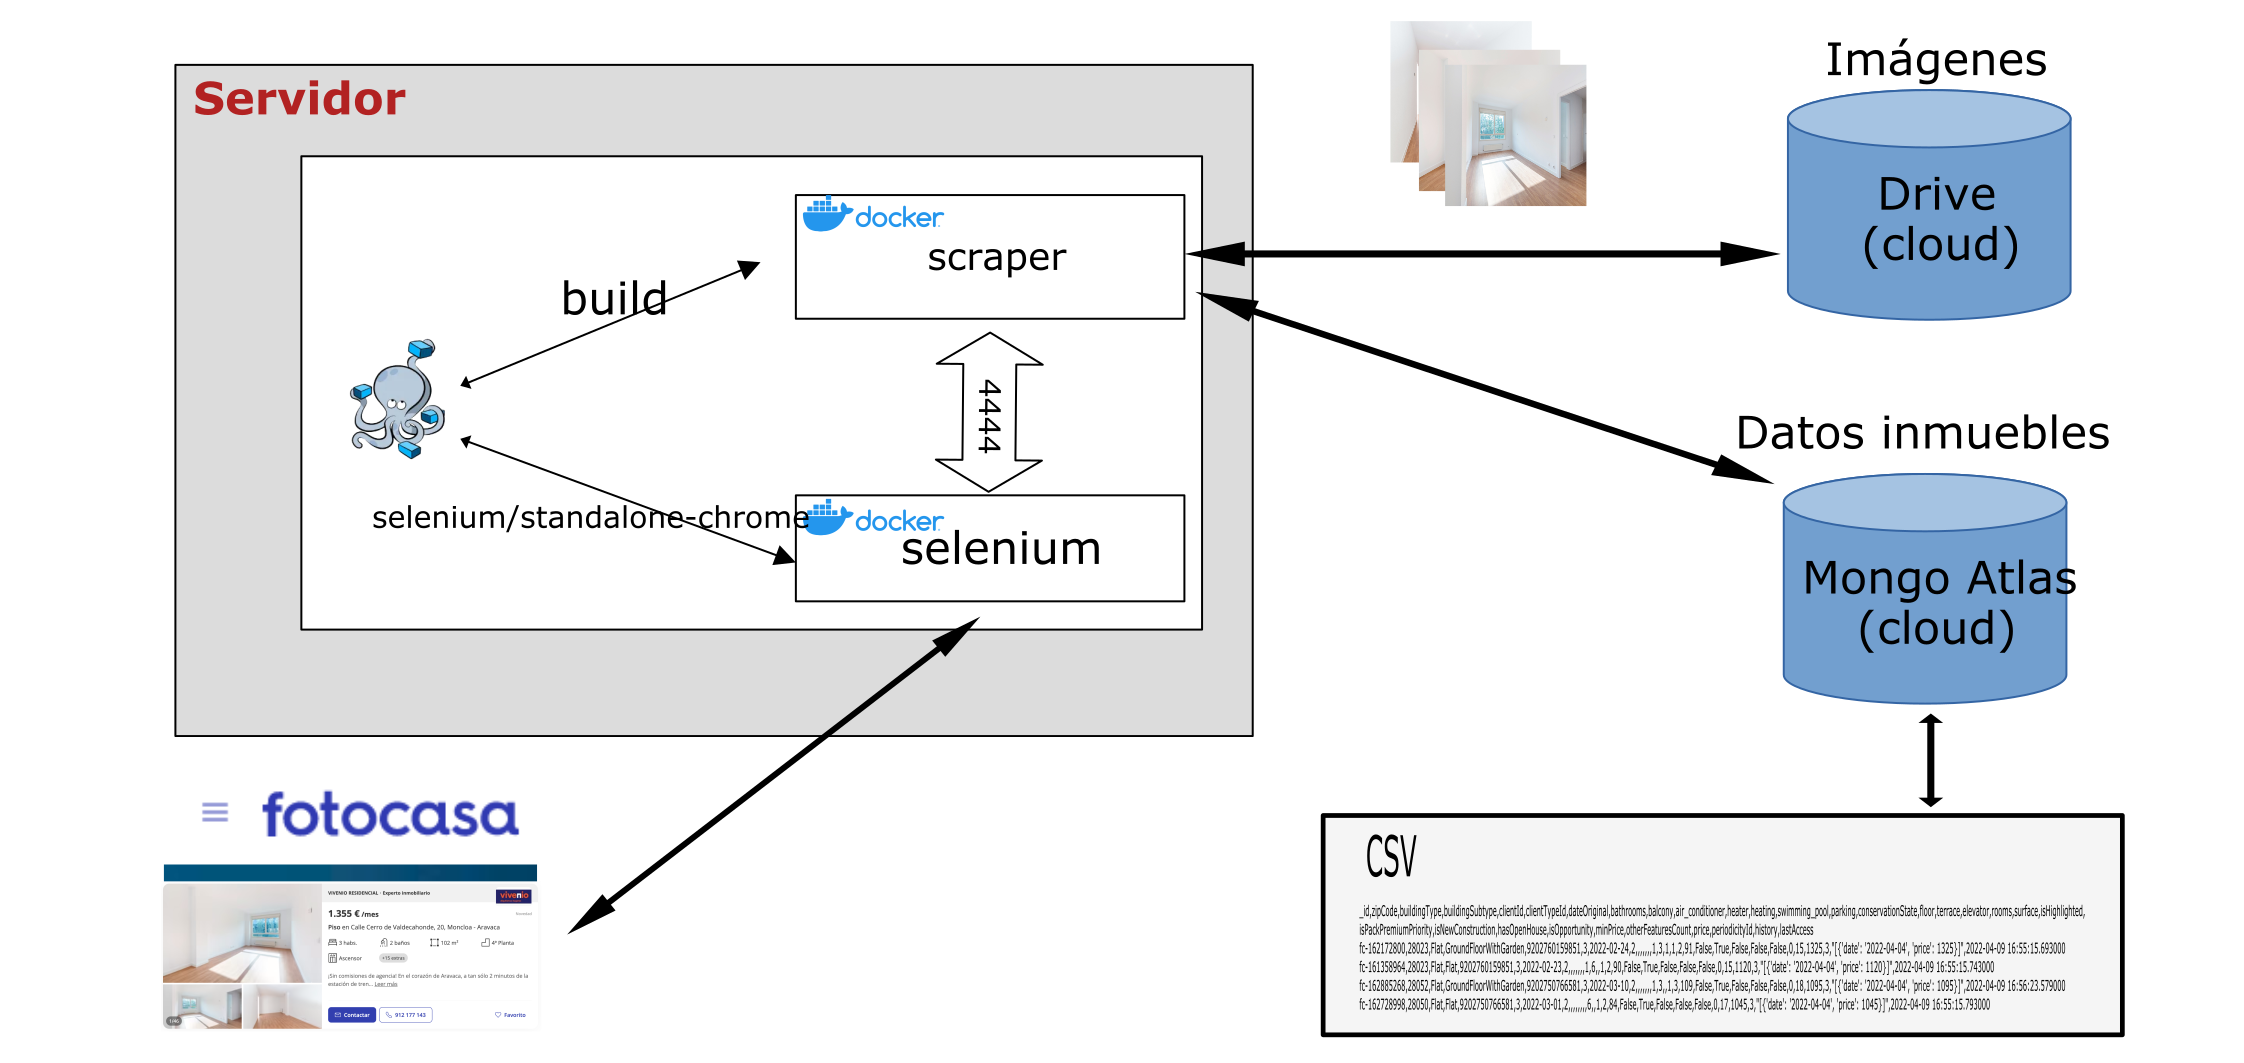
\includegraphics{images/project.png}
\end{figure}

\section{Contenido}

El dataset se encuentra formado por las siguientes características:
\begin{itemize}

	\item \textit{\textbf{id}}: Id. del inmueble, este identificador está anonimizado para que no se pueda asociar al anuncio de origen

	\item \textit{\textbf{zipCode}}: Código postal en el que se encuentra la localidad. Ej: \textit{28023}

	\item \textit{\textbf{buildingType}}: Categoría del tipo de inmueble, en la mayoría de los casos se tratan de pisos (\textit{Flat}).

	\item \textit{\textbf{buildingSubtype}}: Subtipo de inmueble, valor categórico. Ej: \textit{GroundFloorWithGarden}, \textit{Flat}, \textit{SemiDetached}, \textit{Attic}, \dots

	\item \textit{\textbf{clientId}}: Id. del cliente que publica el anuncio. Ej: id-1, id-2, ... 

	\item \textit{\textbf{clientTypeId}}: Categoría del tipo de cliente
	\begin{itemize}
            \item 1: Particular
            \item 2: Inmobiliaria
      \end{itemize}
	\item \textit{\textbf{dateOriginal}}: Fecha de publicación del inmueble. Ej: \textit{2022-03-01}

	\item \textit{\textbf{bathrooms}}: Cantidad de baños (valor numérico). Ej: \textit{2}

	\item \textit{\textbf{balcony}}: Balcón, valor binario tiene o no tiene este extra (\textit{0} ó \textit{1})

	\item \textit{\textbf{air{\_}conditioner}}: Aire acondicionado, valor binario tiene o no tiene este extra (\textit{0} ó \textit{1})

	\item \textit{\textbf{heater}}: Calentador, valor binario tiene o no tiene este extra (\textit{0} ó \textit{1})

	\item \textit{\textbf{heating}}: Calefacción, valor binario tiene o no tiene este extra (\textit{0} ó \textit{1})

	\item \textit{\textbf{swimming{\_}pool}}: Piscina, valor binario tiene o no tiene este extra (\textit{0} ó \textit{1})

	\item \textit{\textbf{parking}}: Parking propio, valor binario tiene o no tiene este extra (\textit{0} ó \textit{1})

	\item \textit{\textbf{conservationState}}: Estado de conservación valor categórico:
	\begin{itemize}
            \item 1: Casi nuevo
            \item 2: Muy bueno
            \item 3: Bueno
            \item 4: A reformar
            \item 8: Reformado
      \end{itemize}
	\item \textit{\textbf{floor}}: Planta en la que se sitúa el piso. Ej: \textit{4}

	\item \textit{\textbf{terrace}}: Terrazas, valor binario tiene o no tiene este extra (\textit{0} ó \textit{1})

	\item \textit{\textbf{elevator}}: Ascensores, valor binario tiene o no tiene este extra (\textit{0} ó \textit{1})

	\item \textit{\textbf{rooms}}: Número de habitaciones. Ej: \textit{3}

	\item \textit{\textbf{surface}}: Superficie de la vivienda en m². Ej: \textit{102}

	\item \textit{\textbf{isHighlighted}}: Valor binario que define si el inmueble está destacado o no (\textit{0} ó \textit{1})

	\item \textit{\textbf{isPackPremiumPriority}}: Anuncio premium, valor binario (\textit{0} ó \textit{1})

	\item \textit{\textbf{isNewConstruction}}: Es de nueva construcción, valor binario (\textit{0} ó \textit{1})

	\item \textit{\textbf{hasOpenHouse}}: Visita libre, valor binario (\textit{0} ó \textit{1})

	\item \textit{\textbf{isOpportunity}}: Es una oportunidad, valor binario (\textit{0} ó \textit{1})

	\item \textit{\textbf{minPrice}}: Precio mínimo aceptado. Ej: \textit{0}

	\item \textit{\textbf{otherFeaturesCount}}: Cantidad de características adicionales, valor numérico. Ej: \textit{15}

	\item \textit{\textbf{price}}: Precio del alquiler. Ej: \textit{1325}

	\item \textit{\textbf{periodicityId}}: Periodicidad de pago del alquiler.
	\begin{itemize}
            \item 0: Desconocido
            \item 3: Mensual
      \end{itemize}
	\item \textit{\textbf{history}}: Historial de precios del inmueble. Ej: \textit{[{'date': '2022-04-04', 'price': 1120}]}

	\item \textit{\textbf{lastAccess}}: Última fecha de acceso a la obtención de los datos. Ej: \textit{2022-04-09 16:55:15.693000}

\end{itemize}


Además se ha trabajado con las imágenes aunque no se haya unificado con el conjunto de datos por motivos de almacenamiento:

\begin{figure}[H]
      \centering
      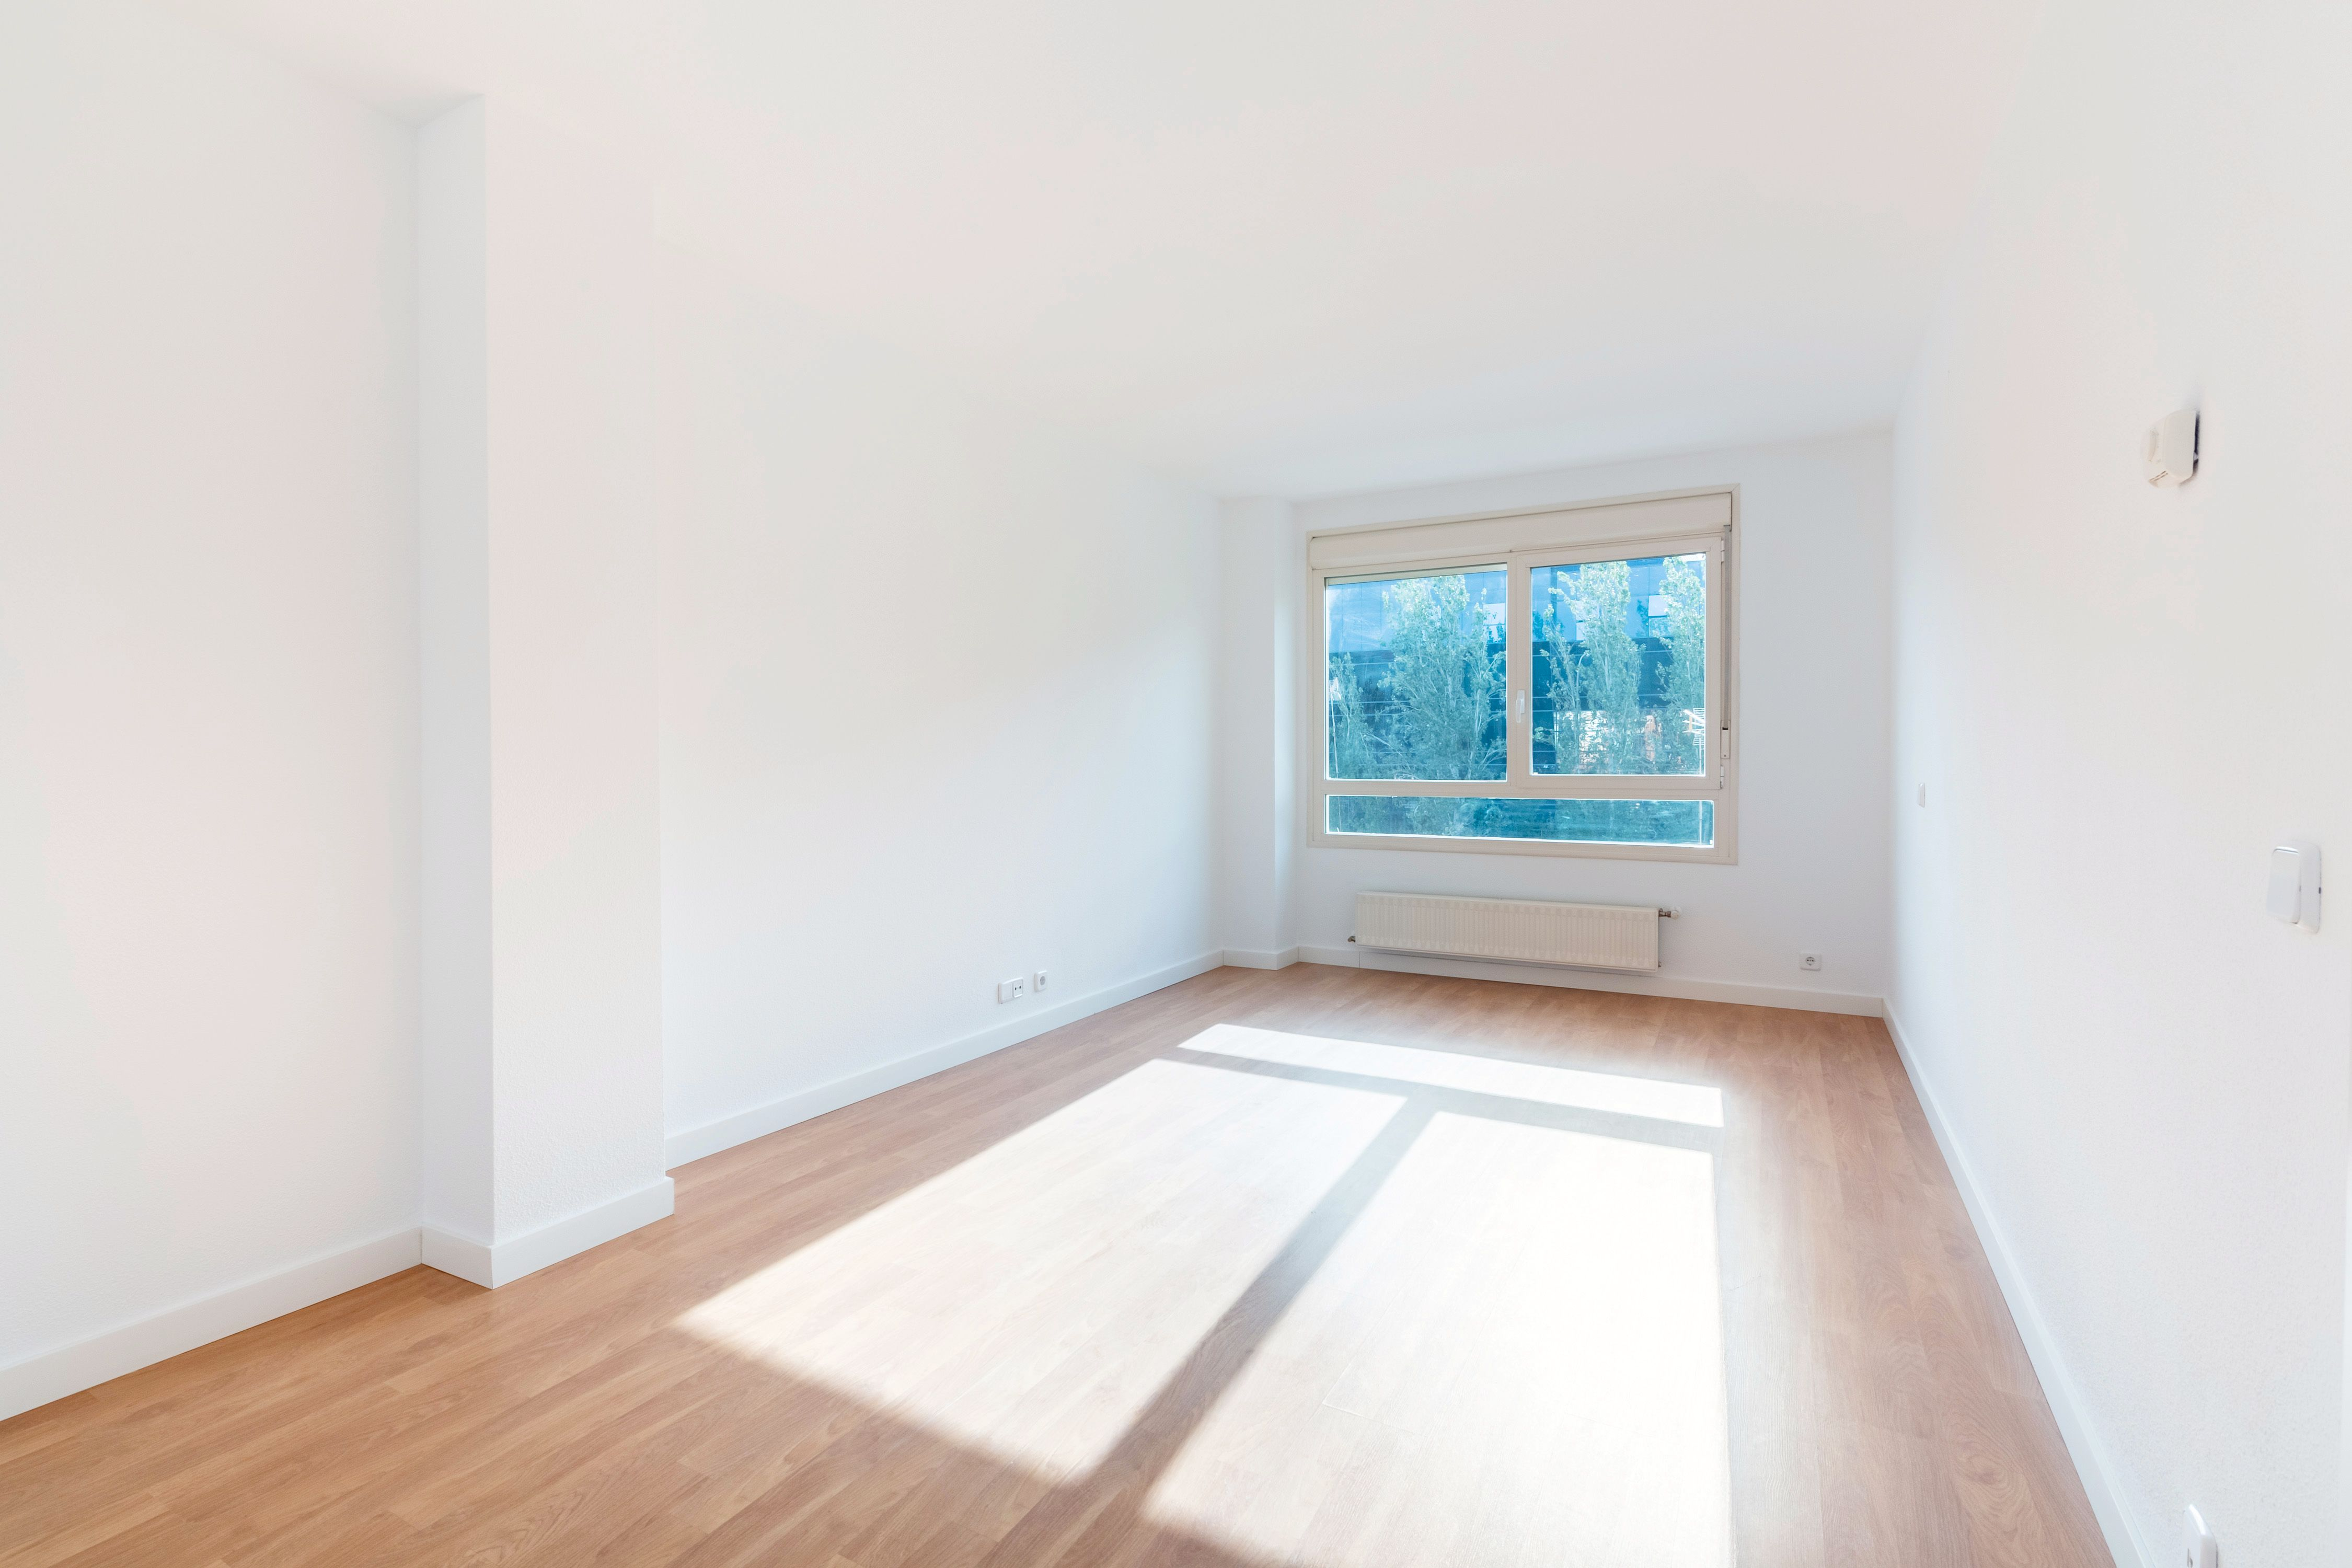
\includegraphics[width=0.7\textwidth]{images/downloaded examples/fc-162706645-466660935.jpg}
      \caption{Imagen extraída automáticamente de la web \href{https://www.fotocasa.es/es/}{Fotocasa}}
      \source{\href{https://static.inmofactory.com/images/inmofactory/documents/1/111353/30315808/466660935.jpg?rule=web_948x542}{Imagen Fotocasa}}
\end{figure}

\section{Agradecimientos}

Específicamente el conjunto de datos obtenido se ha generado, como se comentó en secciones anteriores, de la plataforma de 
venta y alquiler de viviendas \href{https://www.fotocasa.es/es/}{Fotocasa}. Gracias al enfoque de servicios que presenta nos 
ha permitido definir diversas características para obtener todos los datos mediante técnicas de scraping y conseguir obtener 
el conjunto de datos aquí presente. Siguiendo los modelos que presentan este tipo de plataformas para anonimizar su 
localización dentro de los datos recolectados se han obviado algunos como podrían ser cualquier aspecto con el que se 
pueda obtener la dirección real del establecimiento. Todo con el fin de que esto no pueda generar ningún problema al 
proceso de alquiler o al actual propietario. A parte de este tipo de información el resto de atributos se consideran dentro 
de los principios éticos y legales del contexto del proyecto.

\section{Inspiración}

El fin de trabajar con estos datos es por el potencial que presentan. De similar forma existen otros conjuntos de datos los 
cuales tienen unas similares características pero están enfocados en una mayor medida a el precio de venta de determinadas 
viviendas, podemos ver un ejemplo en el conjunto de datos 
\textit{\href{https://www.kaggle.com/c/house-prices-advanced-regression-techniques}{House Prices - Advanced Regression Techniques}} 
de Kaggle. En este, como su título indica se busca aplicar técnicas de regresión para predecir los precios de una vivienda según 
sus características.

En nuestro caso, no sólo se busca poder responder a estas cuestiones, si no que se planean otras como podrían ser la predicción 
del tiempo que una vivienda estará en alquiler (por esto el motivo de registrar los datos existentes en diferentes fechas). Con 
esto se podría optimizar el tiempo de publicación de los anuncios, destacando los parámetros que influyen en mayor medida para 
que un alojamiento sea alquilado en un determinado periodo de tiempo.

\section{Licencia}

Dentro de las licencias establecidas para su publicación se le ha asignado la \textbf{\href{https://creativecommons.org/licenses/by-sa/4.0/deed.es}{CC BY-SA 4.0 License}}. El motivo de aplicar 
este tipo de licencia es que permite el uso de la obra, incluyendo en esto su modificación pero destacando que la autoría 
original tiene que estar presente definiendo así cualquier cambio o transformación realizada en el conjunto de datos. Además, 
por el potencial que observamos en los datos para su uso comercial permitimos así su uso en este contexto.

\section{Código}

El código para generar el correspondiente conjunto de datos se ha realizado mediante el lenguaje de programación Python. 
Este se encuentra disponible en el siguiente \href{https://github.com/jvruoc/rent_prices}{repositorio de Github}. 
En el README principal de dicho repositorio se describen detalladamente las carpetas y códigos existentes que lo 
forman, además de las diversas formas de ejecución desarrolladas y otras notas importantes al trabajar con este proyecto.

\section{Dataset}

Finalmente, el resultado final del dataset se puede encontrar en Zenodo a través 
de \href{https://doi.org/10.5281/zenodo.6445011}{DOI 10.5281/zenodo.6445011}

\section{Contribuciones}

En este apartado se reflejan las contribuciones realizadas por cada uno de 
los autores en las diversas tareas realizadas. Las iniciales en la sección 
de firma representan la confirmación por parte del autor de su participación 
en el apartado correspondiente.

\noindent
\begin{tabular}{@{}ll@{}}
\toprule
      Contribución& Firma\\ 
\midrule
      Investigación previa & V. R., J. - M.Ch., K.\\
      Redacción de las respuestas & M.Ch., K. - V. R., J. \\
      Desarrollo del código:& \\
      \hspace{3mm}- User-agent aleatorio & M.Ch., K.\\
      \hspace{3mm}- Pruebas con proxies & V. R., J. \\
      \hspace{3mm}- Gestión de los elementos dinámicos & M.Ch., K. - V. R., J. \\
      \hspace{3mm}- Descarga de imágenes y subida a Google Drive & M.Ch., K.\\
      \hspace{3mm}- Obtención de características & M.Ch., K. - V. R., J. \\

      Base de datos MongoDB Atlas (carga y extracción) & V. R., J. \\
      Dockerización de la aplicación & V. R., J. \\
\bottomrule
\end{tabular} 



